% Page style for this chapter
	\pagestyle{fancy}
	\lhead{{\sffamily \MakeUppercase{7. Cochlear Vasculature}}}
	\chead{}
	\rhead{{\sffamily \MakeUppercase\rightmark}}
	\lfoot{}
	\cfoot{{\sffamily \thepage}}
	\rfoot{}
	
\chapter{The Role of the Cochlear Vasculature in Volume Conduction}
\label{sect:vascular_structure}

% Textbox
\begin{center}
	\begin{tcolorbox}[title=\boxtitle]
		\begin{itemize}[leftmargin=*,labelindent=2ex,labelsep=1.5ex,itemsep=0pt,parsep=0pt]
			\item What role do blood vessels play in volume conduction?
			\item How strongly do they affect the current pathways?
			\item Should vascular structures be modelled?
		\end{itemize}
	\end{tcolorbox}
\end{center}

%% ================================================================= Vasculature

\section{Introduction}

The cardiovascular system plays a vital role in providing oxygen and nutrients
to almost every cell in the body while also removing metabolic waste products.
Oxygenated blood leaves the heart and is distributed around the body via the
arteries of the systemic circuit. These branch off to supply specific regions
and organs. Smaller arterial branches, known as arterioles, eventually give way
to capillaries, where nutrient, gas, and waste exchange actually takes place.
The morphology then reverses, with the capillaries merging into progressively
larger venules and veins until they re-enter the heart. Deoxygenated blood is
then pumped through the pulmonary circuit, and the cycle begins anew.

The histological structure of each vessel type depends on its function. For
instance, arteries must withstand high, cyclically-loaded intraluminal
pressures, so they are elastic and have a thicker muscle layer. On the other
hand, capillaries only possess thin endothelial linings, which may contain
\emph{fenestrations} (pores) to facilitate chemical exchange with surrounding
cells~\cite{martini2006,mondy2009thesis}.

Like other organs, the cochlea is highly vascularised (recall
\S\ref{sect:cochlear_vessels}). Anatomical studies of the cochlear vessels have
revealed that the network of blood vessels in the inner ear is both pervasive
and delicate~\cite{smith1951,axelsson1968,nakashima2003,roland2006,wright2013}.
The role of these vessels under electrical stimulation has been speculated over
since the pioneering experiments of von \bekesy{}. He observed a multitude of
vessels in the bony wall of the scalae~\cite[p. 659]{vonbekesy1960}, and
suggested that they may be one of the main pathways from the cochlea to the rest
of the body. Resistance results from the Johnstone model~\cite{johnstone1966}
indicated that the vascular pathways are indeed measurably more conductive than
others in the model, but the simple lumped element nature of this model was
unable to reveal any meaningful spatial insights. Girzon did not include any
vascular structures in his volume conduction model (VCM)~\cite{girzon1987},
suggesting that they were ``probably represented adequately\ldots by lumping the
nerve tissue and blood vessels together". He mused that nerve was the main
grounding pathway due to its larger volume, but called for further investigation
of the vasculature as well as the well-supplied spiral ligament. Whiten's
VCM~\cite{whiten2007} included the nearby carotid artery but none of the
internal cochlear vessels. He also speculated that they do not form a
substantial exit pathway, but could not rule out the possibility due to the
known connectivity with larger vessels, such as the carotid artery and jugular
vein.

% Girzon, page 69 - See Schuknecht, 1974; spiral ligament
% Girzon, page 34--35; because nerve volume is larger than blood vessels, the
% major grounding pathway is through the nerve.

The early calls for further investigation were never truly answered, with all
other modelling efforts neglecting the vascular pathways and simply assuming
that they play a negligible role despite the lack of conclusive evidence. As
such, this assumption has remained untested, which is undesirable for a couple
of reasons. Firstly, blood is one of the most conductive tissues in the cochlear
region due to the presence of electrolytes and charged proteins in the plasma
(cf. Figure~\ref{fig:bloodcomp} and
Table~\ref{table:gp_domains})~\cite{gabriel1996b,grimnes2000}. The sprawling
vascular network passes through almost all of the other cochlear tissues, which
have quite different---and often substantially higher---electrical
resistivities. Since current is known to follow the path of least resistance,
these vascular shortcuts may be an important route for intracochlear currents.
Preliminary studies using the proof of concept model~\cite{wong2012} and the
finding by Tran~\etal{} that the jugular vein is an important extracochlear
current pathway~\cite{tran2011,tran2013embc} lend further weight to this idea.

\begin{figure}[t]
	\centering
	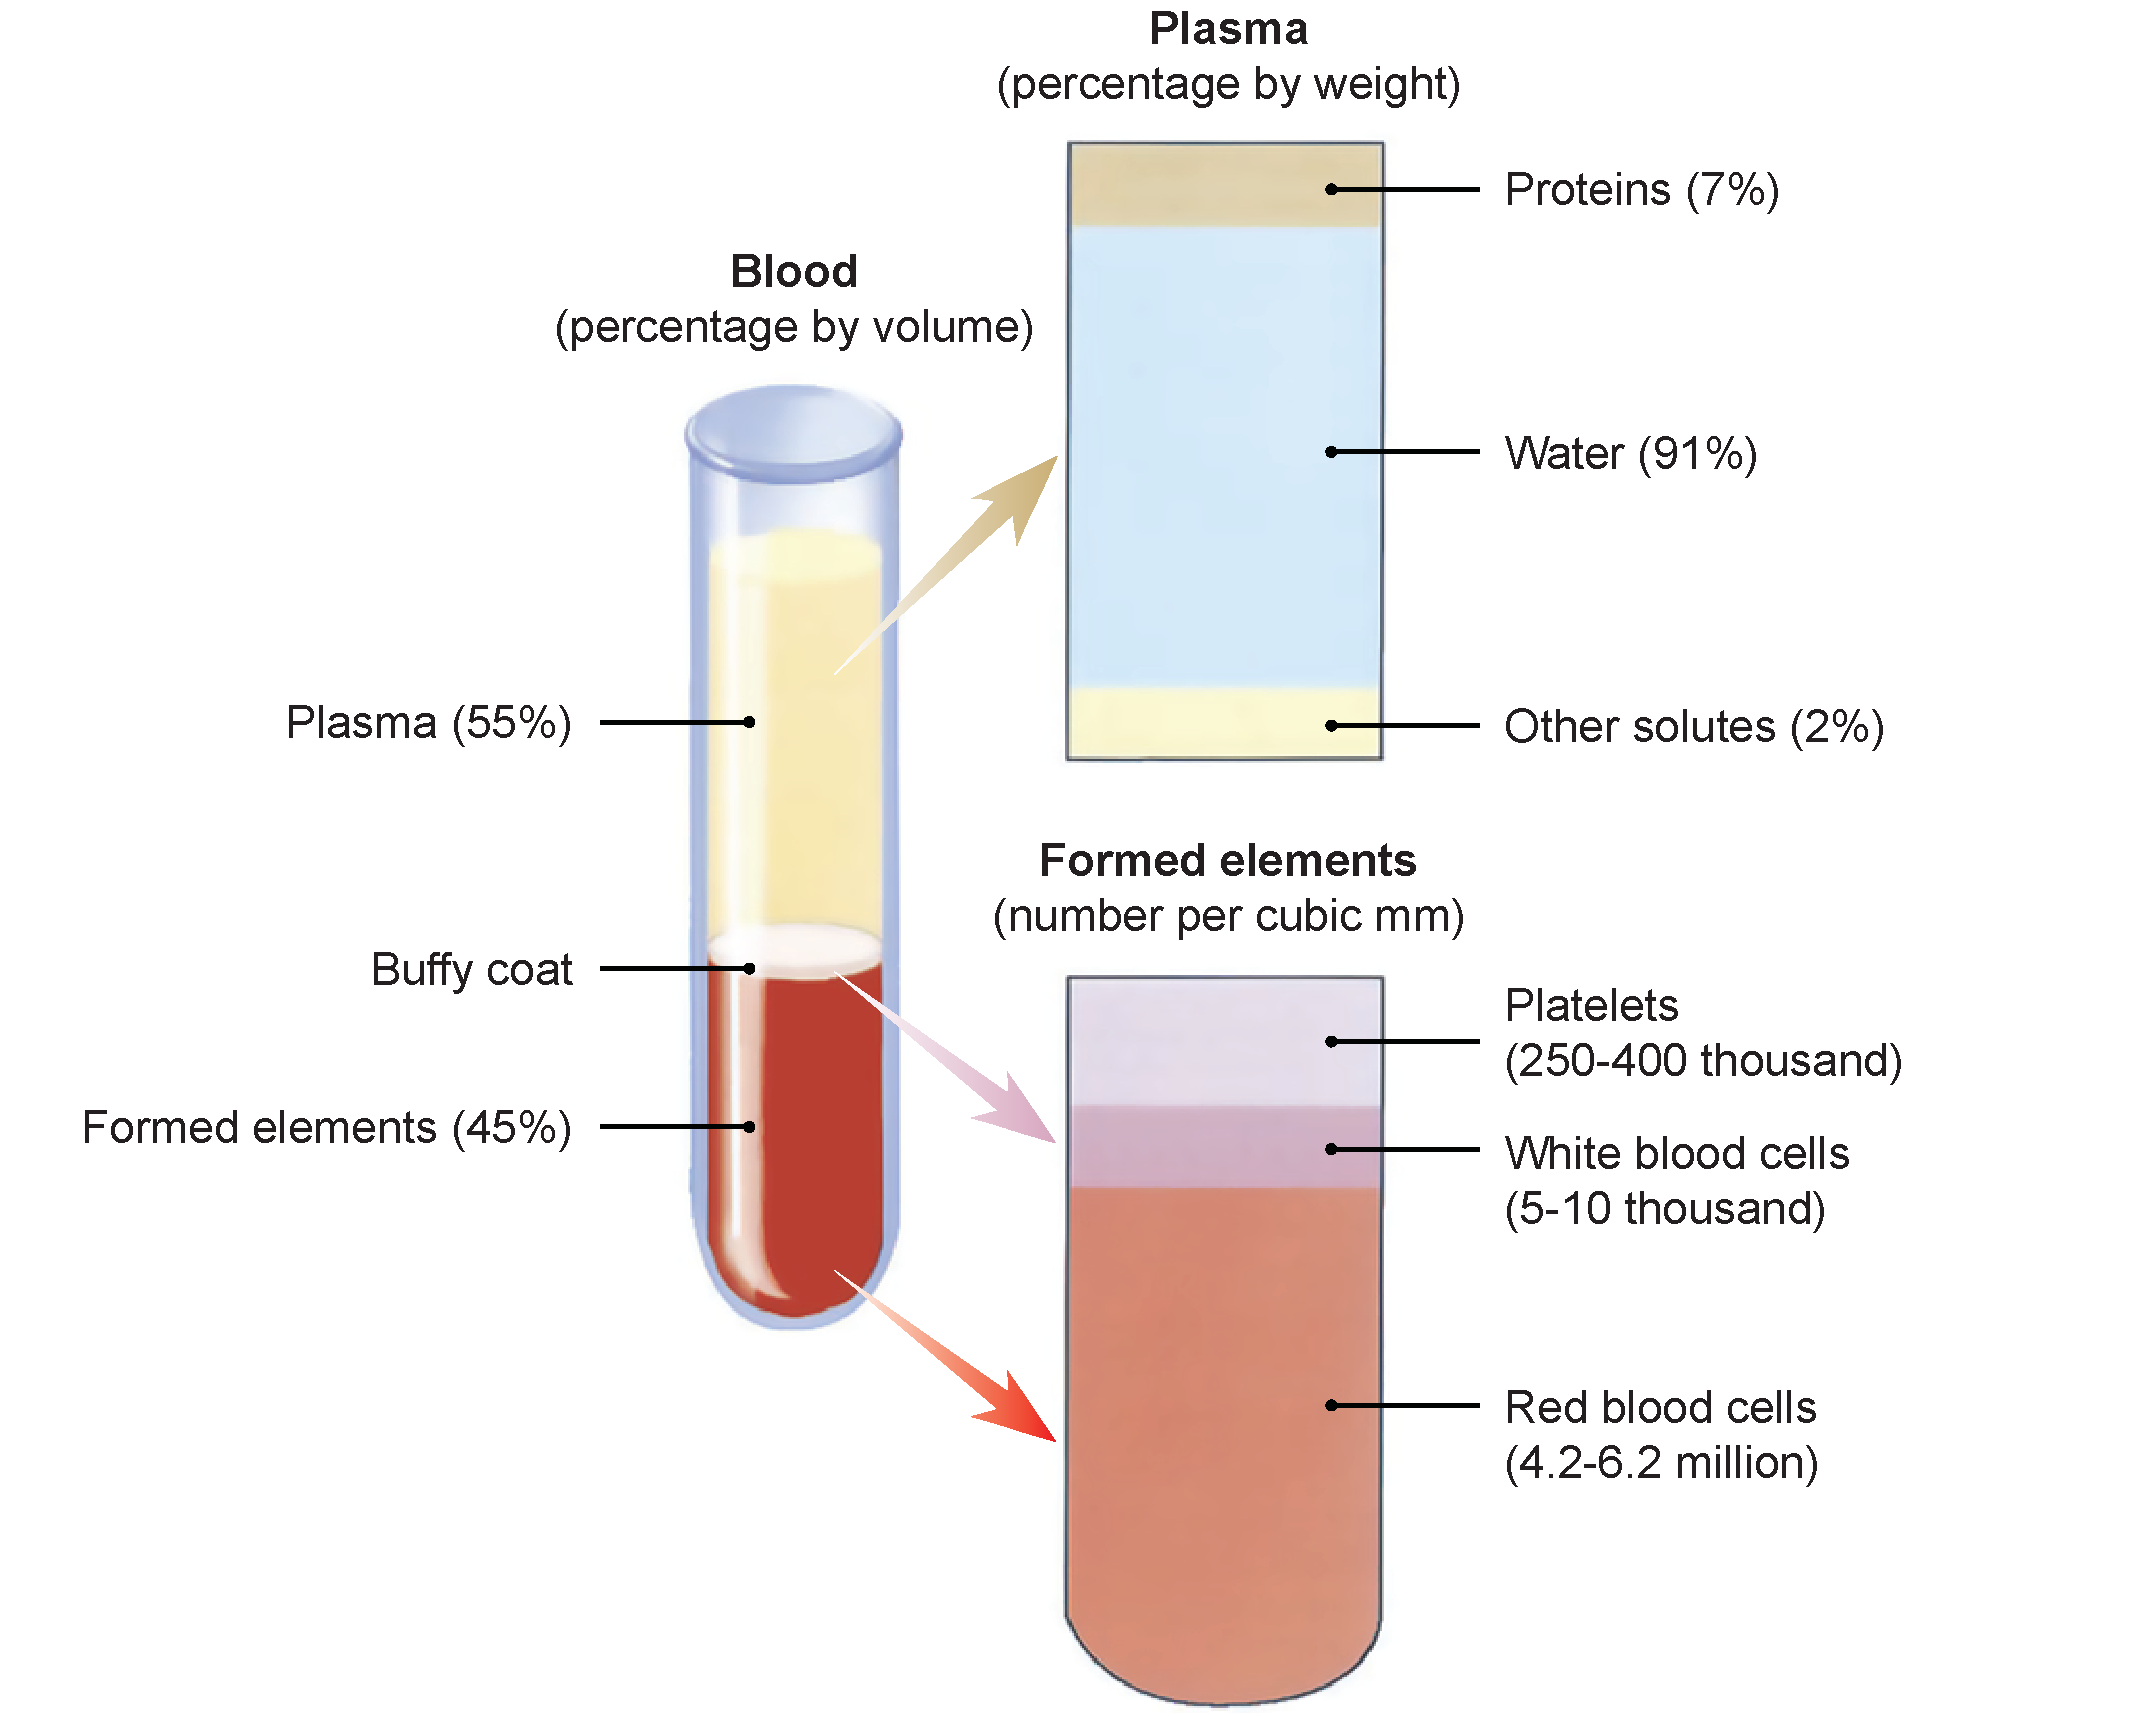
\includegraphics[height=11cm]{Simulations/Vasculature/bloodcomp}
	\caption[The composition of blood]{The composition of blood. (Adapted from
	Tate~\etal~\cite{tate2012}. Copyright \textcopyright{} 2012, McGraw-Hill.)}
	\label{fig:bloodcomp}
\end{figure}

Secondly, the major cochlear vessels---namely the spiral modiolar artery (SMA)
and the vein of the scala tympani (VST)---lie very close to the modiolar wall,
in between the intracochlear electrodes and the neural tissue. This proximity to
the current source means that the vessels may have a more profound impact on the
current pathways than sheer volume alone would suggest, as per the discussion in
\S\ref{sect:expected_physics}~\cite{baker1989}. Even if the differences are
mainly localised and do not have a large bearing on the exit pathways, it would
be prudent to attain a sense of the sensitivity of the model to the vasculature
since it is the current distribution in this main region of excitation that
determines the dominant neural response.

% The proximity of several vessels to other low resistance
% pathways~\cite{nakashima2003} Histological images from Wright show that some
% cochlear blood vessels are directly exposed to the scala. Add images?

Imaging and reconstruction of blood vessels are possible using contemporary
techniques. Studies of larger vessels, such as those in the
heart~\cite{bishop2010} and lungs~\cite{johnson1998} are actually quite common.
Smaller vessels and even entire capillary beds have also been reconstructed
successfully~\cite{ross1995,muller2006blood,mondy2009thesis,wagner2011}.
However, most studies involve organs other than the cochlea, are usually on
non-human species, and generate reconstructions that are suitable for
visualisation but do not meet the more stringent requirements for finite element
(FE) modelling.

The absence of vasculature in existing VCMs of the cochlea suggests that there
may be technical barriers to incorporating them. Perhaps the foremost concern is
spatial resolution because most of the vessels in the cochlea are quite narrow
(see Table~\ref{table:vessel_diams}). The inherent trade-off between resolution
and field of view during the scanning process may make it difficult to
see the entire vascular tree~\cite{muller2006blood,mondy2009thesis}. This is
particularly problematic for human cochleae simply because of their relatively
large size~\cite{thorne1999}.

Another problem is that of contrast. M{\"u}ller found that even with the
resolution advantages of synchrotron radiation-based microCT, the difference in
absorption between the blood vessels and their surrounding tissues was very
small, so the use of appropriate contrast agents is
required~\cite{muller2006blood}. Associated with this is a need for a reliable
staining protocol, made difficult in the cochlea by the lack of physical access
to the site. Even perfusion-based methods cannot guarantee that the vessels will
show up in the scans with complete connectivity~\cite[Fig.~5]{muller2006blood}.

If these imaging challenges can be overcome, then a viable FE model of the
vascularised cochlea may be possible. This would address the existing knowledge
gap and provide a greater understanding of the role played by the cochlear
vessels during electrical stimulation, which may in turn reveal further insights
into the variability between cochlear implant (CI) recipients, or help to
improve future intracochlear electrode array designs and surgical techniques.

\section{Method}

Previous investigations of the cochlear vasculature have made use of a technique
known as \emph{vascular corrosion casting}~\cite{shatari1994,mudry2009}. This
involves injecting a polymer into the bloodstream, which solidifies \invivo{}.
The organ of interest is then extracted from the body and the surrounding tissue
is removed using a corrosive chemical, revealing the hardened polymer in the
shape of the underlying blood vessel network~\cite{hossler2001}. These are then
typically imaged using \emph{scanning electron microscopy} (SEM).

Although such SEM images are great for illustrating the morphology of vascular
networks, they only provide a 2D view of the anatomy. In order to create a 3D
reconstruction, a volumetric dataset is more appropriate. Mondy detailed how
computer models might be obtained from a vascular corrosion cast using
microCT~\cite{mondy2009paper,mondy2009thesis}. Unfortunately, that methodology
results in a free-standing vascular tree model, which is not integrated with the
surrounding tissues and cannot therefore be used to study the volume conduction
problem.

\subsection{MicroCT Imaging with Microfil}

To overcome these limitations, a new imaging protocol was developed in the hopes
of obtaining a scan that was suitable for a complete reconstruction of the
cochlea. A collaboration was established with Ian Curthoys from the School of
Psychology and Christopher Wong from the Australian Centre for Microscopy and
Microanalysis (ACMM), both at the University of Sydney. The general idea was to
fill the blood vessels of the guinea pig cochlea with a radiopaque polymer,
similar to the corrosion casting methods. Instead of eroding the surrounding
tissues however, the specimen would be scanned with all tissues intact.

\subsubsection{Perfusion}

The guinea pig perfusion was conducted according to the standard ethics approval
(University of Sydney Animal Ethics Committee approval L29/4-2010/3/5266). The
animal was deeply anaesthetised with Nembutal and perfused with 400~mL of saline
containing heparin, followed by 500~mL of phosphate buffered Karnovsky's
fixative (3.5\% paraformaldehyde and 0.5\% glutaraldehyde). This perfusion
technique has been shown to cause minimal distortion to the delicate cochlear
membranes at the electron microscope level~\cite{anniko1977}.

At the same time, the injection compound was prepared. In this case, Microfil by
Flow Tech Inc. was used. This compound was selected for its radiopacity, which
allowed it to serve as a contrast agent for microCT imaging. The yellow MV-122
variant was procured as a kit and approximately 20~mL of the compound was
prepared according to the standard mixing procedure (see
Appendix~\ref{appendix:microfil_specs}).

The chest of the guinea pig was opened and the heart was exposed. A cannula was
inserted into the left ventricle and the descending aorta was clamped. The
curing agent was then added to the mixture of MV-122 and diluent and the
Microfil was injected into the cannula after ensuring that there were no air
bubbles in the syringe. The animal was left in place overnight to allow the
Microfil to set. After this, the temporal bone was removed (see
Figure~\ref{fig:microfil_perfusion}) and wrapped in parafilm with phosphate
buffer solution.

\begin{figure}
    \centering
    \begin{subfigure}[t]{0.5\textwidth}
        \centering
        \includegraphics[height=4.6cm]{Simulations/Vasculature/26-05-12-18-24-05}
        \caption{}
        \label{fig:microfil_bulla}
    \end{subfigure}%
	\hfill%
	\begin{subfigure}[t]{0.5\textwidth}
        \centering
        \includegraphics[height=4.6cm]{Simulations/Vasculature/15-05-12-09-53-19}
        \caption{}
        \label{fig:microfil_apex}
    \end{subfigure}\\%
    \vspace{1em}
	\begin{subfigure}[t]{0.5\textwidth}
        \centering
        \includegraphics[height=4.6cm]{Simulations/Vasculature/26-05-12-17-47-56}
        \caption{}
        \label{fig:microfil_lateral}
    \end{subfigure}%
    \hfill%
    \begin{subfigure}[t]{0.5\textwidth}
        \centering
        \includegraphics[height=4.6cm]{Simulations/Vasculature/15-05-12-09-59-48}
        \caption{}
        \label{fig:microfil_radiating}
    \end{subfigure}\\%
    
	\caption[Perfusion of the guinea pig cochlea using Microfil]{Perfusion of the
	guinea pig cochlea using Microfil (yellow). The compound appears to have filled
	most of the vessels along the surface of the bone at the very least. (a) The
	perfused cochlea within the exposed tympanic bulla; (b) the apex of the perfused
	cochlea; (c) the vessels along the outer surface of the otic capsule; (d) the
	radiating arterioles at the apical turn. The Microfil in the radiating
	arterioles suggests that the modiolar vessels were also successfully perfused.}
	\label{fig:microfil_perfusion}
\end{figure}

\subsubsection{Imaging}

The wrapped specimens were attached to holders and placed within the scanning
chamber of an Xradia MicroXCT-400 (Xradia, CA, USA; recently bought out by
Zeiss). To ensure optimal acquisition of the images through the utilisation of
maximum dynamic range, the scanning parameters for each specimen were
individually optimised. For the actual acquisition of the 3D dataset, the
specimens were scanned incrementally over 360 degrees in steps of approximately
0.2 degrees for a total of 1800 x-ray images. In general, the exposure time for
each image was about 30--40 seconds. The tomographic dataset was then
reconstructed using the local hardware-based back projection reconstruction
software supplied by Xradia. This produced a 16-bit, $ 1024 \times 1024 \times
1024 $ voxel image stack with a resolution of 11~$ \upmu $m in each direction.

Initial scans lacked contrast between the tissues, so additional staining was
performed. Both the oval window and a semicircular canal were penetrated to
facilitate diffusion of the stains through the volume. The specimens spent up to
6 days in ethylenediamine tetra-acetic acid (EDTA) for bone
decalcification~\cite{schneider2009} and another 2 days in osmium tetroxide
(\ce{OsO4}) to enhance the soft tissues~\cite{wong2013}. Typical scan results
are shown in Figure~\ref{fig:microfil_microCT}.

\begin{figure}[t]
    \centering
	
	\begin{subfigure}[t]{0.5\textwidth}
        \centering
        \includegraphics[height=7.5cm]{Simulations/Vasculature/microfil_vessels_video}
        \caption{After 6 days in EDTA}
        \label{fig:microfil_vessels}
    \end{subfigure}%
    \hfill%
	\begin{subfigure}[t]{0.5\textwidth}
        \centering
        \includegraphics[height=7.5cm]{Simulations/Vasculature/volren_15000-18500}
        \caption{After another 2 days in \ce{OsO4}}
        \label{fig:microfil_volren}
    \end{subfigure}%
	
	\caption[Visualisation of the vascular network in the guinea pig
	cochlea]{Visualisation of the vascular network in the guinea pig cochlea. (a)
	Reconstruction of the vessels only using the Xradia software, showing that the
	vascular tree was extensive but not perfectly perfused. (b) Volume rendering
	in Amira after additional soft tissue staining shows the VST spiralling around
	the cochlear nerve trunk.}
	\label{fig:microfil_microCT}
\end{figure}

The protocol was able to produce a spectacular and insightful map of the
cochlear vasculature, and the results presented here represent the first time
the cochlear vasculature has been imaged in microCT with such detail \insitu.
However, a couple of shortcomings ultimately ruled out reconstruction using this
dataset. Figure~\ref{fig:microfil_microCT} shows that despite the care taken
throughout the experiment, some of the vessels appeared to be disconnected,
potentially due to microbubbles or clotting. The microCT images were also not as
clear as the alternative sTSLIM dataset (which were received part way through
this experiment) for showcasing all of the cochlear tissues. Although
segmentation of the blood vessel network would have been substantially quicker
with the Microfil data, it was judged that a better overall model could be
achieved by using the sTSLIM scans.

\subsection{Reconstruction from sTSLIM}

The sTSLIM data, as discussed previously in \ref{sect:sTSLIM_imaging}, provided
an ideal combination of resolution and clarity, and revealed an unprecedented
amount of structural detail. However, it was difficult to ascertain the
locations of the cochlear vessels from the images themselves because previous
reports~\cite{axelsson1968,nakashima2003} were largely schematic---they did not
illustrate the vessel trajectories in the context of the surrounding tissues
clearly, nor did they reveal their true (often convoluted) shape. With the
microCT map of the vessels serving as a reference, the cochlear vessels could be
segmented from the sTSLIM images with more certainty. In this way, the high
resolution sTSLIM images were combined with the high contrast microCT data to
enable a more accurate reconstruction of the vascularised guinea pig cochlea.

In terms of practicality, two simplifications were made. The first was
that only the larger blood vessels were segmented, because it was likely that
the finer branches of the vascular tree, especially those further from the
current source, would only have a small effect on volume conduction. In order to
test this hypothesis, three levels of detail were modelled:
\begin{description}%[after=\vspace{1.5\medskipamount}]
	\item[\textsf{BV0}] No blood vessels, analogous to
	existing VCMs.
	\item[\textsf{BV1}] Major vessels only, i.e. the SMA, VST,
	vestibulo-cochlear vein (VCV), and the vein of the cochlear aqueduct (VCAQ).
	\item[\textsf{BV2}] Major vessels with visible primary branches, including the
	``vascular spring-coils''~\cite{scuderi1952} or glomeruli~\cite{franz1993}
	extending from the SMA, and the vein of the round window (VRW).
\end{description}

These three cases are illustrated in Figure~\ref{fig:vasc_detail}. For each
case, the blood vessels were segmented independent of the other cochlear tissues
(i.e. as separate layers), and only the relevant masks for each level of detail
were made visible during the surface reconstruction process in ScanIP. This
allowed for a \textit{ceteris paribus} comparison of the VCM with and without
blood vessels. An attempt was made at including the radiating arterioles because
their trajectories could be discerned in the sTSLIM images. Unfortunately the
arterioles were only a few voxels wide in the images, which made them extremely
difficult to segment accurately. Given that this would have complicated the
subsequent discretisation steps, it was decided not to include them in this
study.

\begin{figure}
	\centering
	
	\begin{subfigure}[t]{0.31\textwidth}
        \centering
        \includegraphics[height=6cm]{Simulations/Vasculature/GP_noBV_trans10}
        \caption{BV0}
        \label{fig:vasc_noBV}
    \end{subfigure}%
    \hfill%
    \begin{subfigure}[t]{0.31\textwidth}
        \centering
        \includegraphics[height=6cm]{Simulations/Vasculature/GP_mainBV}
        \caption{BV1}
        \label{fig:vasc_mainBV}
    \end{subfigure}%
    \hfill%
    \begin{subfigure}[t]{0.31\textwidth}
        \centering
        \includegraphics[height=6cm]{Simulations/Vasculature/GP_allBV}
        \caption{BV2}
        \label{fig:vasc_allBV}
    \end{subfigure}%
    
    \caption[Levels of detail for the vascularised reconstruction]{Levels of
    detail for the vascularised reconstruction. (a) The unvascularised model
    (BV0); (b) the model with major vessels only (BV1); (c) the model with major
    vessels in addition to some primary branches (BV2).}
	\label{fig:vasc_detail}
\end{figure}

The second simplification was that the vessel walls were ignored. The main
reason for this was that they could not be distinguished clearly in the sTSLIM
images. Even if they could be segmented, they would be extremely difficult to
discretise. Considering that the resistivity of blood vessel walls has been
estimated to be about two to four times that of blood~\cite{edgerton1975}, which
would put their electrical response close to that of the surrounding tissue, and
that they are thin relative to the lumen (which are already quite narrow), the
vessel walls were not expected to have a large effect.

The simulations for this study were set up as in previous investigations, with
material properties per Table~\ref{table:gp_domains}, a 1~mA current source
injected at electrode E4, and the voltage offset boundary condition applied at
the temporal bone surface.

\section{Results}

\subsection{Degrees of Freedom and Solution Times}

Unsurprisingly, the number of degrees of freedom (DOFs) increased with the
amount of vascular detail as shown in Table~\ref{table:bv_solution_times}.
Using quadratic discretisation, the unvascularised model resulted in just over 5
million DOFs. Adding the main vessels and additional branches required another
1.1 million and 900,000 DOFs respectively. Solution times using the Conjugate
Gradient solver were quite reasonable, with all three simulation cases
completing in about 80 minutes.

\begin{table}
	\centering
	\sffamily
	\small
	
	\caption[Degrees of freedom and solution times for the vascularised
	models]{Degrees of freedom and solution times for the vascularised
	models.}
	\label{table:bv_solution_times}
	
    \begin{tabular}{l r r}
		\toprule
		\textbf{Level of detail~~~~}	& \textbf{Degrees of freedom}
			& \textbf{~~~~~Solution time} \\
		\midrule
		
		BV0	&	5,132,816	& 21 mins 54 secs \\
		BV1	&	6,277,592	& 27 mins 23 secs \\
		BV2	&	7,140,772	& 31 mins 17 secs \\
		\bottomrule
	\end{tabular}
	\bigskip
\end{table}

\subsection{Voltage along the Array}

Voltages measured along the intracochlear electrode array were highly
insensitive to vascular detail. A plot showed the traces as overlapping, so the
data were tabulated (Table~\ref{table:vasc_voltages}) and the deltas plotted
(Figure~\ref{fig:bv_tv_delta}). These show there was very little difference
between the three cases, with average deltas of only -0.23\% and -0.12\% for BV1 and BV2
respectively relative to the unvascularised BV0 case. In fact, the largest delta
at any point was only -0.51\%, observed at the stimulating electrode E4 in the
BV2 case, well below the Frijns sufficiency criterion~\cite{frijns1995} used
previously.

\begin{table}
	\mathversion{sans}
	\centering
	\sffamily
	\small
	\caption[Voltages along the array]{Voltages along the array. Percentage
	differences were calculated relative to BV0.}
	\label{table:vasc_voltages}
	
	\begin{tabularx}{0.75\textwidth}{X c c c c c}
		\toprule
		\textbf{Electrode}	& \textbf{BV0}	& \multicolumn{2}{c}{\textbf{BV1}} &
			\multicolumn{2}{c}{\textbf{BV2}} \\
		& \textbf{Voltage (V)} & \textbf{Voltage (V)}	& \textbf{$
			\mathsf{\boldsymbol{\Delta}} $ (\%)} & \textbf{Voltage (V)}	& \textbf{$
			\mathsf{\boldsymbol{\Delta}} $ (\%)} \\
		\midrule
		
		\csvreader[late after line=\\]%
			{Simulations/Vasculature/voltage_profiles.csv}%
			{1=\electrode,2=\nobv,3=\mainbv,4=\mainbvdelta,5=\allbv,6=\allbvdelta}%
 			{\electrode & \nobv & \mainbv & \mainbvdelta & \allbv & \allbvdelta}%
		\bottomrule
	\end{tabularx}
	
\end{table}

\begin{figure}
	\centering
	\includegraphics[height=7cm]{Simulations/Vasculature/bv_delta}
	\caption[Effect of vascular detail on intrascalar voltages]{Effect of vascular
	detail on intrascalar voltages. Percentage deltas are relative to BV0 as per
	Table~\ref{table:vasc_voltages}.}
	\label{fig:bv_tv_delta}
\end{figure}

\subsection{Current Pathways}

\begin{figure}[p]
	\centering
	
	\begin{subfigure}[t]{0.45\textwidth}
        \centering
        \includegraphics[height=7cm]{Simulations/Vasculature/streamlines-BV-noBV-blank}
        \captionsetup{margin={-0.5cm,0cm}}
        \caption{BV0}
        \label{fig:vasc_streams_noBV}
    \end{subfigure}%
    \begin{subfigure}[t]{0.45\textwidth}
        \centering
        \includegraphics[height=7cm]{Simulations/Vasculature/streamlines-BV-allBV-blank}
        \captionsetup{margin={-0.5cm,0cm}}
        \caption{BV2}
        \label{fig:vasc_streams_allBV}
    \end{subfigure}%
    \hfill%
    \begin{subfigure}[t]{0.09\textwidth}
        \centering
        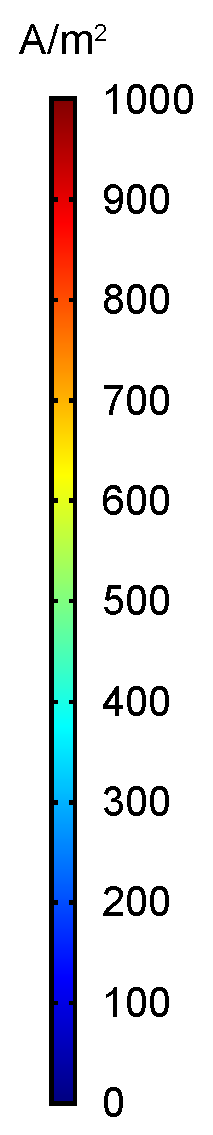
\includegraphics[height=7cm]{Simulations/Vasculature/cbar_streamlines}
    \end{subfigure}%
    
    \caption[Comparison of exit pathways]{Comparison of exit pathways. There
    was very little difference between the two cases. Current appeared to veer
    slightly closer to the modiolus due to the lower resistance posed by the
    blood vessels, especially towards the apical end.}
	\label{fig:vasc_streams}
\end{figure}

\begin{figure}[p]
	\centering
	
	\begin{subfigure}[t]{0.44\textwidth}
        \centering
        \includegraphics[height=7cm]{Simulations/Vasculature/heatmap-BV-noBV-edit}
        \caption{BV0}
        \label{fig:vasc_heat_noBV}
    \end{subfigure}%
    \hfill%
    \begin{subfigure}[t]{0.44\textwidth}
        \centering
        \includegraphics[height=7cm]{Simulations/Vasculature/heatmap-BV-allBV-edit}
        \caption{BV2}
        \label{fig:vasc_heat_allBV}
    \end{subfigure}%
    \hfill%
    \begin{subfigure}[t]{0.09\textwidth}
        \centering
        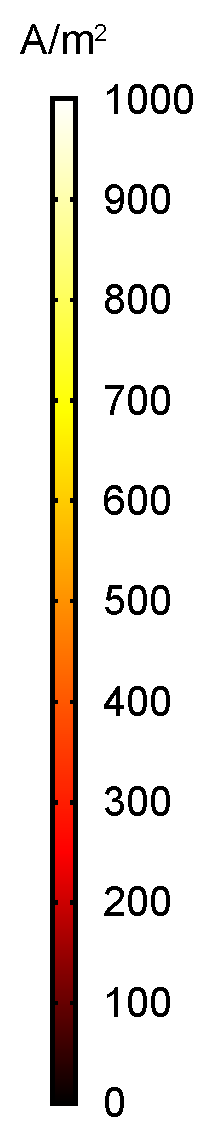
\includegraphics[height=7cm]{Simulations/Vasculature/cbar_heatmap}
        \label{fig:vasc_heat_cbar}
    \end{subfigure}%
    
    \caption[Comparison of current density heatmaps]{Comparison of current
    density heatmaps. The BV2 case shows current density that is elevated in
    some regions (e.g. the VST, circled in green), but lower in others (e.g.
    vessels in the CSF, circled in blue). Note that the current source is
    behind the mid-modiolar slice shown here.}
	\label{fig:vasc_heatmaps}
\end{figure}

Adding vasculature to the model only appeared to have a small effect on the
conduction pathways as well. The streamlines in Figure~\ref{fig:vasc_streams}
show that the apical exit pathways moved slightly towards the modiolus when
vascular pathways were included, but the overall pattern was largely similar
between the BV0 and BV2 cases. This is likely because the effects were
predominantly localised to the regions near the blood vessels, as shown in
Figure~\ref{fig:vasc_heatmaps}. Changes in the current distribution depended on
the tissue surrounding the vessel. Those passing through bone saw an increase in
local current density due to the lower resistivity of blood. Vessels passing
through cerebrospinal fluid (CSF) experienced the opposite because the
surrounding tissue was more conductive.

It was of particular interest to see how the current density in neural
structures was affected. The current density in Rosenthal's canal (JRC) for the
three test cases is tabulated in Table~\ref{table:vasc_jrc} and the deltas
plotted in Figure~\ref{fig:bv_jrc_delta}. JRC was more sensitive to the vascular
detail than suggested by the previous results for voltage profiles and exit
pathways. Peak JRC values were 0.90--1.76\% lower than in the unvascularised
model. More dramatic changes were seen at an insertion angle of 298 degrees,
half a turn deeper than the stimulating electrode, where the deltas were
5.5--7\%. The average change over all sample points was less than 1.5\%,
indicating that the differences were quite localised. For the most part, the
vascularised models predicted lower JRC values than the unvascularised model,
adding weight to the view that blood vessels are a preferred pathway.

\begin{table}
	\mathversion{sans}
	\centering
	\sffamily
	\small
	\caption[Current density in Rosenthal's canal]{Current density in Rosenthal's
	canal. As before, the deltas were calculated relative to BV0.}
	\label{table:vasc_jrc}
	
	\begin{tabularx}{0.76\textwidth}{X c c c c c}
		\toprule
		\textbf{Insertion angle}	& \textbf{BV0}	& \multicolumn{2}{c}{\textbf{BV1}} &
			\multicolumn{2}{c}{\textbf{BV2}} \\
		\textbf{(Degrees)}	& \textbf{JRC (\nicefrac{A}{m\textsuperscript{2}})}	&
			\textbf{JRC (\nicefrac{A}{m\textsuperscript{2}})}	& \textbf{$
			\mathsf{\boldsymbol{\Delta}} $ (\%)}	& \textbf{JRC
			(\nicefrac{A}{m\textsuperscript{2}})}	& \textbf{$
			\mathsf{\boldsymbol{\Delta}} $ (\%)} \\
		\midrule
		
		\csvreader[late after line=\\]%
			{Simulations/Vasculature/jrc.csv}%
			{1=\angle,2=\nobv,3=\mainbv,4=\mainbvdelta,5=\allbv,6=\allbvdelta}%
 			{\angle & \nobv & \mainbv & \mainbvdelta & \allbv & \allbvdelta}%
		\bottomrule
	\end{tabularx}
	
\end{table}

\begin{figure}
	\centering
	\includegraphics[height=7cm]{Simulations/Vasculature/jrc_delta}
	\caption[Effect of vascular detail on current density in Rosenthal's
	canal]{Effect of vascular detail on current density in Rosenthal's
	canal. Percentage deltas are relative to BV0 as per
	Table~\ref{table:vasc_jrc}.}
	\label{fig:bv_jrc_delta}
\end{figure}

\subsection{Activating Function}

Variations in neural current density and current pathways were both small when
measured independently. However, the likelihood of excitation as measured using
the activating function (AF) was more substantial because it effectively
considers both quantities in tandem. AF results for all three cases are given in
Figure~\ref{fig:vasc_af}, and once again, there were indications of localised
differences along the neural sheet. The region nearest to the stimulating
electrode saw a substantial increase in depolarisation at the nodes of Ranvier
immediately neighbouring the VST. The nodes slightly further out from there saw
a mild reduction in depolarisation. Deeper nodes from more apical axons one turn
away also experienced a large increase in AF, highlighting the importance of
considering the 3D structure of the cochlea. In both of these regions, the level
of depolarisation was slightly shifted towards the axonal end, as expected given
the location of the VST and its effect on the local current paths.

\begin{figure}
	\centering
	
	\begin{subfigure}[t]{0.3\textwidth}
        \centering
        \includegraphics[height=4.5cm]{Simulations/Vasculature/2D-AF-BV-noBV}
        \caption{BV0}
        \label{fig:vasc_af_noBV}
    \end{subfigure}%
	\begin{subfigure}[t]{0.3\textwidth}
        \centering
        \includegraphics[height=4.5cm]{Simulations/Vasculature/2D-AF-BV-mainBV}
        \caption{BV1}
        \label{fig:vasc_af_mainBV}
    \end{subfigure}%
	\begin{subfigure}[t]{0.3\textwidth}
        \centering
        \includegraphics[height=4.5cm]{Simulations/Vasculature/2D-AF-BV-allBV}
        \caption{BV2}
        \label{fig:vasc_af_allBV}
    \end{subfigure}%
    \begin{subfigure}[t]{0.09\textwidth}
        \centering
        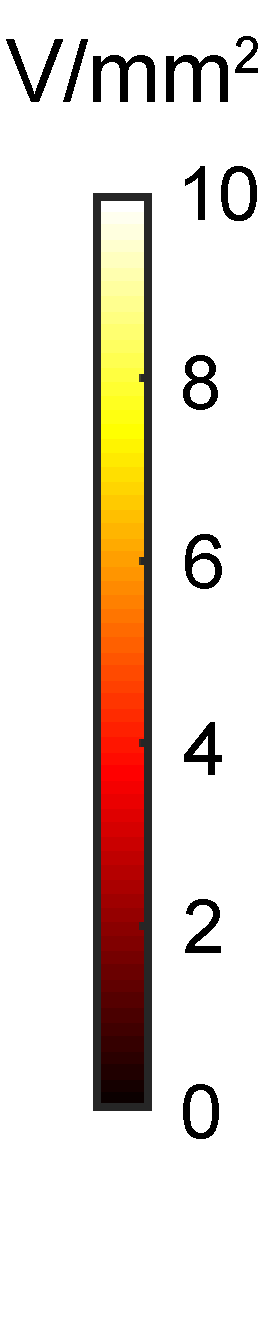
\includegraphics[height=4.77cm]{Simulations/Vasculature/cbar_af_abs}
        \label{fig:vasc_af_noBV_cbar}
    \end{subfigure}\\%
    
    \vspace{1em}%
    \begin{subfigure}[t]{0.3\textwidth}
    	\phantom{\hspace{4.73cm}}
    \end{subfigure}%
    \begin{subfigure}[t]{0.3\textwidth}
        \centering
        \includegraphics[height=4.5cm]{Simulations/Vasculature/delta_AF-BV-mainBV}
        \caption{BV1}
        \label{fig:vasc_af_delta_mainBV}
    \end{subfigure}%
    \begin{subfigure}[t]{0.3\textwidth}
        \centering
        \includegraphics[height=4.5cm]{Simulations/Vasculature/delta_AF-BV-allBV}
        \caption{BV2}
        \label{fig:vasc_af_delta_allBV}
    \end{subfigure}%
    \phantom{\hspace{3.42mm}}%
    \begin{subfigure}[t]{0.09\textwidth}
        \centering
        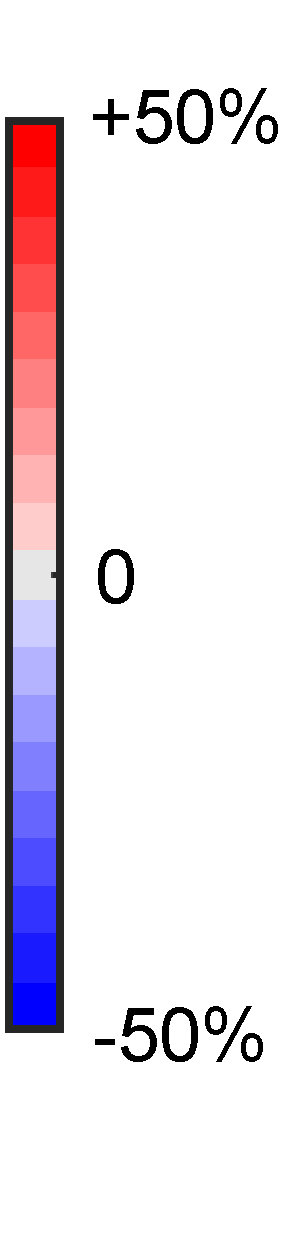
\includegraphics[height=4.5cm]{Simulations/Vasculature/cbar_af_delta}
        \label{fig:vasc_af_delta_cbar}
    \end{subfigure}%
    
    \caption[Effect of vascular detail on the activating function]{Effect of
    vascular detail on the activating function. Absolute value of the
    computed AF for (a) the unvascularised case, (b) with the main vessels, and
    (c) with the additional branches. Percentage differences along the neural
    sheet (relative to BV0) are also shown for the latter two cases in
    subfigures (d) and (e), with RMS deltas in the top right corner.
    It appears that the presence of the main modiolar vessels has a funnelling
    effect on nearby current, leading to more depolarisation in the neural
    tissue immediately surrounding it. The effect is very localised but can
    affect the axons of more apical neurons as they pass through the region of
    influence. Additional fine detail had little marginal impact in this study.}
	\label{fig:vasc_af}
\end{figure}

To quantify the overall level of activity, the root mean square (RMS) value of
AF was calculated for each case. Differences in these RMS values, reported in
the delta plots in Figure~\ref{fig:vasc_af}, confirmed that the general pattern
was mostly unchanged, with deltas below 1.5\%. Both vascularised cases predicted
a net reduction in overall depolarisation compared with the unvascularised
model. The AF trend from BV0 to BV1 was slightly reversed by the additional
detail of BV2, indicating that the changes are not due to volume of tissue
alone. However, in the region closest to the stimulating electrode, the
marginal impact of additional vasculature always increased the AF.

\section{Discussion}

Due to the historical development of cochlear models, with lumped element models
(LEMs) evolving into VCMs as technology progressed, many studies have framed the
question of current flow through the tissues as ``either/or'' in nature. Unlike
in an electrical circuit though, where current is restricted to flowing through
wires and elements, current in the cochlea flows volumetrically and can pass in
and out of tissues at any point, with the actual path determined by the overall
spatial distribution of the conductive medium. As such, there is no single
tissue that can be thought of as \emph{the} exit pathway, and in determining the
role of the cochlear vasculature, it is worth considering both local and global
perspectives.

\subsection{Local Effects}

From the results, it was clear that the AF is more sensitive to the presence of
the vasculature than suggested by the negligible changes in intrascalar
voltages. The difference in resistivity between the blood and the immediately
surrounding tissue was a key driver of the local current distribution.
Streamlines emanating from the stimulating electrode were densest near the
electrode itself, so the major vessels in the nearby modiolus had the strongest
influence on the results, as predicted by Baker~\cite{baker1989}.

For insertions in the scala tympani, the vessel of primary interest was the VST,
which lies in the modiolar wall where it meets the floor of the scala tympani.
The presence of the VST diverted some of the current that normally flows through
the spiral ganglion cells. This shift in the local pathway indicated that the
blood provided a lower resistance alternative. It reduced the level of
depolarisation at nodes of Ranvier nearest the spiral ganglion while elevating
depolarisation at nodes further down the axon (see Figure~\ref{fig:vasc_af}).
The differences were smaller toward the basal end but neurons from more apical
turns were affected because their axons passed through the region of influence.
More advanced neural excitation models may be sensitive to the changes brought
on by the inclusion of the blood vessels.

A corollary of these findings is that the presence of the cochlear vasculature
has a greater impact in simulations with modiolar-hugging electrode arrays than
those with more lateral designs. Current injected nearer to the modiolus is more
likely to encounter and be diverted by the VST, so optimising the alignment of
the platinum pads relative to the modiolus (e.g. by changing the orientations of
the exposed platinum surfaces and/or ensuring that they are slightly angled
towards the apex during insertion) may increase current flow and depolarisation
in the spiral ganglion cells, and could potentially reduce ectopic stimulation
of more apical fibres. Further simulations would need to be conducted before
such effects can be confirmed.

Insertions in the scala vestibuli are less common in clinical practice and were
not directly studied here. However, given the simulation results, it can be
expected that the SMA and its branches would be the key vessels to consider in
those cases. The impact is expected to be weaker than that observed in scala
tympani insertions because although the arteries still lie between the scala and
the nerve tissue, they are thinner, more distant from the scala, and are
surrounded by the highly conductive CSF.

\subsection{Global Effects}

The study demonstrated that in general, the blood vessels have little bearing on
the dominant patterns in the cochlea. Voltages in the scala tympani exhibited
negligible change, which may have attributed to early experimental findings that
the vasculature could be ignored. Both voltages and JRC were slightly lower in
the vascularised models (Tables~\ref{table:vasc_voltages} and
\ref{table:vasc_jrc}), which was expected because the vessels have a lower
resistivity than their surrounding tissues. RMS values for the AF also did not
change much beyond the regions of the neural sheet near the current source. This
provides some affirmation for existing cochlear models that have omitted the
vascular structures.

The only substantial changes in regions further from the stimulating electrode
were almost exactly half a turn away in the apical direction
(Table~\ref{table:vasc_jrc}). This can be explained by the current flowing in
that direction encountering more of the modiolar vessels, with a cumulative
effect from the localised distortions in current density. However, JRC and AF
magnitudes were significantly lower there than at the peak, so the absolute
deltas are not expected to result in large changes in neural excitation at those
neurons. On a related note, there appeared to be a correlation between JRC and
AF in these data. This provides some support for the finding by
{\AA}str{\"o}m~\etal{} that computational neuron models may not be required for
predicting excitation in certain types of investigations~\cite{astrom2014}.

These findings may be relevant to other neuroprosthetic devices that involve
electric current injection in close proximity to vascular structures, such as
subretinal or suprachoroidal retinal prostheses~\cite{guenther2012}. \textit{In
silico} studies of those implants would be advised to include the larger
vascular structures at the very least as part of the anatomical reconstruction.

\subsection{Study Limitations}

Aside from the issues mentioned previously under
\S\ref{sect:validation_discussion}, the main limitation specific to this study
is that of detail. Most of the vessels that were included in this study were
located in the modiolus because the larger size of these vessels made them
relatively easy to segment and mesh, and their proximity to both the current
source and the neural structures justified the effort required to reconstruct
them. However, Figures~\ref{fig:siebenmann} and \ref{fig:microfil_microCT}
illustrate that the modelled vascular tree was far from complete. With time, it
may be possible to include the radiating arterioles in addition to other
peripheral vessels, and perhaps also model the vessel walls using simple mask
dilation techniques (only the lumen is represented in these models). However,
judging from the results of this study, it would seem that the additional time
and computational resources required to produce and analyse a
vasculature-complete model is not warranted.

\section{Conclusions}

The addition of the cochlear vasculature did not have a large effect on the
modelling outputs, with the exception of the large vessels in the modiolus where
a strong local effect was observed. In particular, the vein of the scala tympani
was shown to have a substantial impact on activating function in the surrounding
neural tissue due to its large size and close proximity to the current source.
It diverted some of the injected current away from the spiral ganglion, which
caused changes in the activating function distribution along the neural sheet.
In that sense, the vascular pathways offered a preferred low resistance pathway
over the nerve tissue in that region.

Considering the substantial additional effort required to incorporate the
vascular structures and the overall small impact on the end results, it is
recommended that future models wishing to add vascular detail focus their
efforts on the vein of the scala tympani only. The localised changes arising
from this vessel alone may prove important for more sophisticated models of
neural excitation.
